\graphicspath{{chapters/_resources/}}

\chapter{Journal Clubs}

\section{Mechansims of transcription regulation}
\subsection{Enhancers are activated by p300/CBP activity-dependent PIC assembly, RNAPII recruitment, and pause release}

E1A binding protein p300/CREB-binding protein is a \emph{transcriptional co-activator} and \emph{histone acetyltransferase}. p300/CBP activity has been directly implicated in enhancer activation through acetylation (H3K27ac hallmark). p300/CBP-catalyzed acetylation promotes the recruitment of BRD4, and therefore the release of promoter-proximal-paused RNAPII. p300/CBP can regulate pro-proliferative pathways.

\textbf{Aim of this article:} investigate the function and mechanisms of p300/CBP-catalyzed acetylation in dynamic enhancer activation.

To analyze the effects of p300/CBP inhibition on enhancers, SILAC (Stable isotope labeling by amino acids in cell culture) can be performed to obtain a relative quantification of A-485-induced acetylome and proteome changes. A-485 is a highly selective inhibitor of p300/CBP catalytic activity. 

Time-resolved nascent transcription analyses in A-485-treated ESCs [5-ethynyluridine sequencing (EU-Seq)] revealed that p300/CBP inhibition causes rapid enhancer deactivation. In addition, p300/CBP inhibition selectively downregulates cell-type-specific (CTS) genes.

TSA, a KDAC inhibitor, is able to fully recover acetylation levels after inhibition. TSA-induced transcription changes are not affected by A-485 co-treatment.

p300/CBP inhibition does not impair TF and p300 binding:
\begin{itemize}
\tightlist
\item increased p300 binding at TSS inversely correlates with reduced expression of downstream genes
\item p300/CBP activity appears to contribute to its dynamic dissociation from chromatin
\item chromatin binding of TFs and p300/CBP per se is not sufficient to activate enhancers
\end{itemize}

To investigate whether A-485-induced transcription inhibition results from a change in chromatin accessibility, ATAC-Seq can be applied to detect chromatin accessibility levels. It was observed that p300/CBP inhibition reduces chromatin accessibility, hence p300/CBP-catalyzed acetylation and/or ongoing transcription likely contributes to chromatin accessibility and rapid transcription inhibition by A-485 is unlikely due to a direct consequence of altered chromatin accessibility.

p300/CBP functions through BET-BRD-dependent and -independent mechanisms, BET inhibitors e.g. JQ1 slightly downregulate A-485 genes, but not as much as A-485. Indeed, p300/CBP activity promotes RNAPII recruitment independently of promoting pause release independently from BRD4.

p300/CBP-catalyzed acetylation promotes TFIID binding and PIC assembly:
\begin{itemize}
\tightlist
\item genes showing a slow TBP and RNAPII dissociation kinetics, such as Scl2a3 and Tfcp2l1, contain
TATA-box
\item genes displaying rapid TBP and RNAPII dissociation such as Nanog, Zfp42 and Esrrb, lack
canonical TATA-box
\item p300/CBP activity regulates the PIC assembly of enhancer-regulated, but not housekeeping genes.
\item reduction in TAF1, TBP and RNAPII binding is positively correlated
\end{itemize}

p300/CBP-catalyzed acetylation is crucial for TFIID anchoring, and, consequently, for PIC assembly and transcription initiation at enhancers and enhancer-regulated genes.

\textbf{Conclusions:}
\begin{itemize}
\tightlist
\item p300/CBP and deacetylase activities regulate dynamic (de) activation of enhancers
\item p300/CBP-catalyzed acetylation promotes PIC assembly and RNAPII recruitment
\item BRD4 acts as a p300/CBP downstream effector to promote RNAPII pause release
\item Coupling of RNAPII recruitment and pause release enables rapid enhancer activation
\end{itemize}

\begin{figure}
\centering
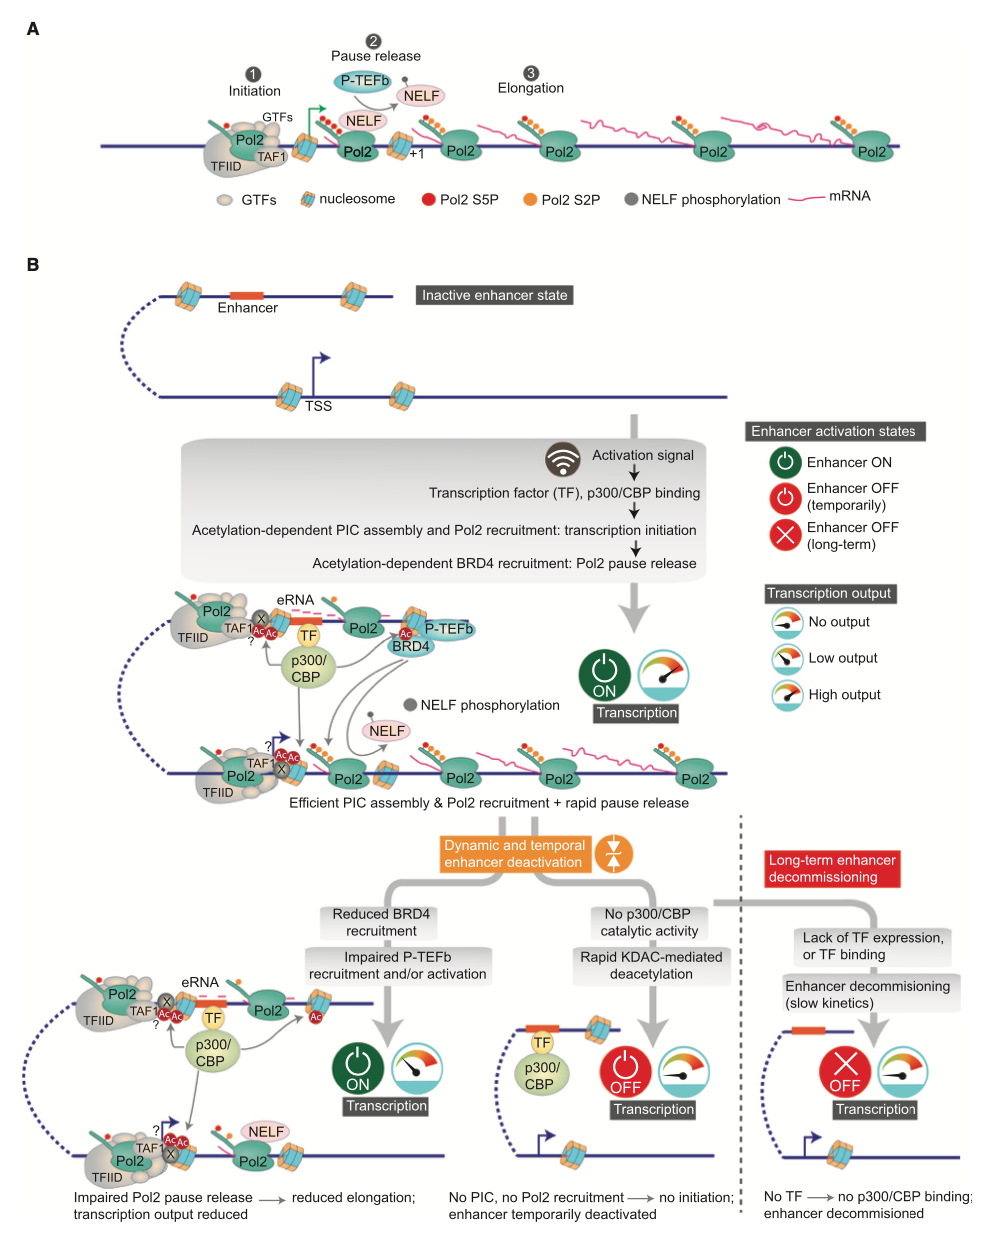
\includegraphics[width=0.7\textwidth]{../_resources/Screenshot_2022-12-19_at_16-39-14.png}
\caption{(A) Schematic depiction of the key steps in the transcription cycle.
(B) Proposed hypothetical model of p300/CBP-activity-dependent dynamic enhancer activation. }
\end{figure}

\subsection{SPT5 stabilization of promoter - proximal RNA polymerase II}
Aoi et al. find that the conserved transcription elongation factor SPT5 stabilizes RNA polymerase II (RNA Pol II) in yeast and human
cells. SPT5 loss triggers degradation of a RNA Pol II subunit through CUL3, VCP, and CDK9. Stabilizing RNA Pol II may be a SPT5’s primary function to safeguard accurate gene expression.

Acute depletion studies: RNAPolII undergoes a 2-step pausing at NELF and at the +1 nucleosome: a depletion of NELF causes the RNAPolII to still be paused at the +1 nucleosome. Additional regulatory mechanism for the release of RNAPolII into the gene body.

SPT5 is an evolutionarily conserved and essential elongation factor. It forms the DSIF complex with SPT4. It interacts with RNAPolII throughout the elongation phase, probably active as a positive elongation factor, but impossible to knock-out.

Depletion of SPT5 through the generation of auxin-inducible degron (AID) avoids effects of long-term depletion and leads to an RBP1 degradation (the largest subunit of Pol II). 

SPT5 physically localizes with RNAPolII at most transcriptionally active genes on chromatin.Therefore, SPT5 depletion may affect the protein-protein interaction properties/composition of RNAPolII transcription units. \textbf{CUL3} is one of the human Cullin family proteins that serve as scaffolds of Cullin-RING E3 ubiquitin ligase complexes. Cul3 knockdown partially stabilized RBP1 upon SPT5 depletion, but did not affect SPT5-AID degradation. Recent studies showed how DNA damage causes RBP1 degradation by NEDD4 or CUL5, but upon SPT5 degradation they did not show any stabilization ability. CUL3- RNAPolII association on chromatin is triggered by SPT5-AID degradation.

\textbf{VPC} is known to mediate the unfolding of ubiquitylated proteins through its ATPase activity leading to efficient protein degradation.
VCP inhibition did not stabilize RBP1 when inhibiting initiation by triptolide (TPL).
There are (at least) two distinct pathways:
\begin{enumerate}
\tightlist
\item VCP-dependent degradation induced by SPT5 depletion
\item VCP-independent degradation induced by a TPL-stimulated initiation effect
\end{enumerate}
RBP1 is degraded either during the early elongation stage at promoter-proximal region, or during the productive elongation stage, in absence of SPT5.

To determine how SPT5 depletion and VCP inhibition affect the steady state of transcription by RNA Pol II, SPT5-AID cells were treated with the VCP inhibitor, followed by auxin, and then ChIP-seq for RNA Pol II was performed. RPB1 degradation induced by SPT5 loss occurs during the early stages of elongation. RNAPolII was able to travel substantial distances when SPT5 was depleted (although the distance was shorter than the control). RNAPolII at the elongation stage is unlikely to be degraded in the absence of SPT5. Even when RNAPolII is stabilized a the promoter-proximal region, it still needs SPT5 for the elongation stage in the body of the gene.

NELF regulates the transition of pausing states. Upon NELF loss, RNAPolII travels from a first pause region to a second pause region corresponding to the +1 nucleosome dyad. The SPT5 depletion system, coupled with the VCP inhibition described earlier, may allow us to precisely
investigate the SPT5 function in promoter-proximal pause/release. They performed precision run-on sequencing (PRO-seq) to map the RNA Pol II positions at base-pair resolution. RNA Pol II was paused at the second pause regions when depleting SPT5 and inhibiting VCP, which resembles NELF depletion.

\textbf{Conclusions:}
SPT5 regulates promoter-proximal pausing at the first pause region, likely through its interaction with NELF, and that the transition to the second pause region upon SPT5 depletion is through NELF dissociating from RNA Pol II.
Two possible roles for SPT5:
\begin{enumerate}
\tightlist
\item SPT5 loss leads to unproductive elongation on nucleosomes, which may trigger RPB1 destabilization.
\item This raises another possibility: that SPT5 may regulate RPB1 stability and
proper elongation (pausing and velocity) independently.
\end{enumerate}

\begin{figure}
\centering
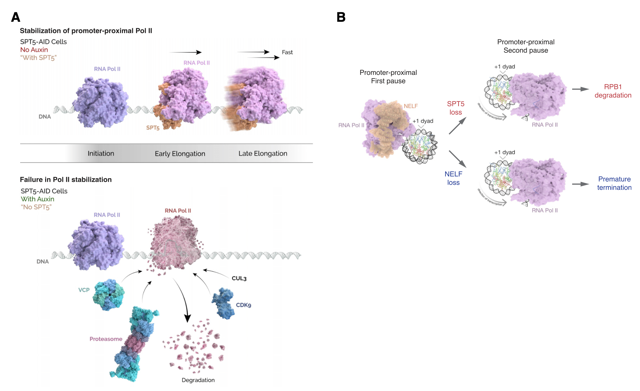
\includegraphics[width=0.8\textwidth]{../_resources/Screen_Shot_2022-12-19_at_17-00-41.png}
\caption{(A) SPT5 stabilizes RNA Pol II during the early elongation stage. With the SPT5 protein (upper panel), once RNA Pol II is initiated and escapes from the promoter, RNA Pol II undergoes productive elongation until termination. Without SPT5 (lower panel), early-elongating RNA Pol II undergoes RPB1 degradation that is mediated by the CUL3 ubiquitin ligase, the VCP unfoldase, and a novel form of the P-TEFb component CDK9. Late-elongating RNA Pol II without SPT5 can persist in transcription at a slower speed.
(B) Failure in RNA Pol II passage on the +1 nucleosome leads to 2 distinct pathways to eliminate RNA Pol II from chromatin.}
\end{figure}

\section{Mechanisms of transcription regulation in cancer}

\subsection{MYC Recruits SPT5 to RNA Polymerase II to Promote Processive Transcription Elongation}

MYC encodes for a nuclear phosphoprotein and is involved in cell cycle progression, apoptosis and cellular transformation. It forms heterodimers with MAX and binds to E-box containing DNA and regulates expression of non-coding transcripts and mRNA expression by RNA pol II.

\begin{figure}
\centering
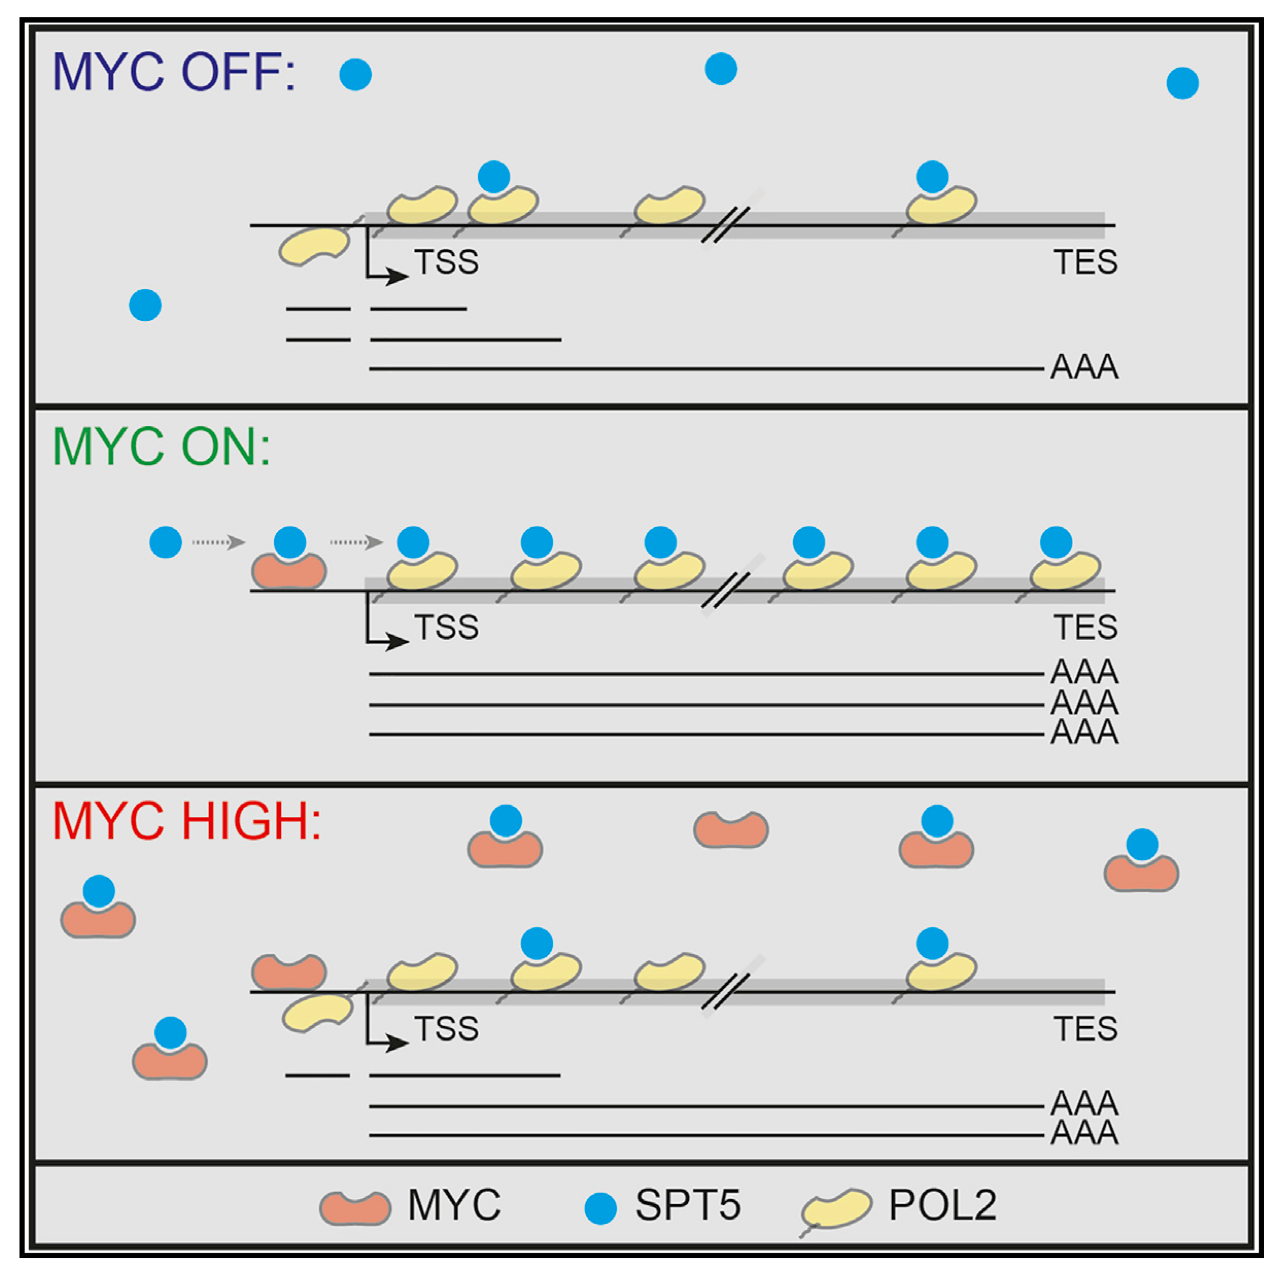
\includegraphics[width=0.3\textwidth]{../_resources/Screenshot_2022-10-28_at_10-37-23.png}
\caption{}
\end{figure}

ChiP-seq analysis revealed that MYC binds at the majority of open promoters. MYC is able to modulate the transcriptional cycle, and two mechanism are
proposed:
\begin{itemize}
\tightlist
\item
  MYC can recruit CDK9 to mediate pause release
\item
  MYC transfers Pol II associated factor PAF1 complex onto Pol II
\end{itemize}

Through the analysis of Tet-Off/On system, it was seen that MYC controls the assembly of transcriptionally engaged pol II complexes.
\begin{itemize}
\tightlist
\item
  6 common proteins in pol II and MYC interactome, but only SPT5 and SPT6 changed their association with Pol II upon MYC depletion
\item
  upon MYC depletion, read distribution at all expressed genes showed a
  global reduction of SPT5 binding → chromatin- associated Pol II binds
  to less SPT5 in the absence of MYC
\end{itemize}

By performing In situ Proximity Ligation Assay (PLA), we can achieve the detection of individual proteins or protein complexes using antibodies attached by DNA strands. PLA between SPT5 and pS2-Pol II shows clear reduction in nuclear proximity pair in absence of MYC in both U2OS and HMLE cells, meaning that upon MYC depletion we observe less interaction among SPT5 and Pol II. 

MYC recruits SPT5 by binding to its N-Terminal region.

CDK7 Activity is Required for Transfer of SPT5 from MYC to Pol II, as MYC facilitates the CDK7-dependent assembly of Pol II-SPT5 complexes.
In addition, MYC Influences Processivity and Directionality of Pol II after pause release:

\begin{itemize}
\tightlist
\item
  Reduced processivity and directionality upon MYC depletion
\item
  MYC Maintains High Pol II Elongation Rates
\item
  Overexpression of MYC has an inhibitory effect on Pol II elongation
  rate. SPT4 is sequestered by MYC, and therefore its binding with Pol
  II is decreased. Certain genes lose processivity and directionality at
  oncogenic levels of MYC → MYC dependent sequestration of SPT5 might
  repress tumor-suppressive genes.
\end{itemize}

MYC is not a pioneer TF, it only binds to accessible binding sites. MYC is able to bind low-affinity binding sites in a scenario of MYC overexpression.


\subsection{BRD4-directed super-enhancer organization of transcription repression programs links to chemotherapeutic efficacy in breast cancer}

BET are epigenetic leaders, they can recognize marks through
bromodomain. \textbf{BRD4} is a positive regulator of transcription. It
is involved in some disorders, as inflammation, obesity and cancer, as
it can enhance the transcription of oncogenes. JQ1 inhibits BET4 and is
a promising antitumor drug, but a resistance can be developed.

\textbf{Super-enhancers} are clusters of enhancers occupied by master
regulators e.g.~BRD4 or Mediator, which control the expression of
lineage-specific genes.
\begin{itemize}
\tightlist
\item
  NuRD complex: multi-subunit, repressor. Acts as chromatin remodeling
  complex and histone deacetylase.
\item
  LSD1: histone demethylase
\item
  Pellino (PEL1): E3 ubiquitin ligase
\end{itemize}

Thanks to MF we can identify interactors: all the components of LSD1/NuRD complex, confirmed
by Western Blotting and coIP assays.BRD4 is directly interacting with LSD1 through the C-terminus.

Interaction with factors known to reside in super-enhancer regions
e.g.~MED-1 was consolidated with ChIP-seq, almost 23000 targets in common.
The sequences bound are enriched in H3Kme1 and H3k27ac.

SE control genes in important signalling pathways and drug resistance e.g.~PDPK1.

After 4 weeks cancer resistant cells emerge. BRD4 is quickly inhibited,
while LSD1 or MTA3 in the early phase of treatment maintain chromatin
contact, which is exactly lost at 4 weeks.
\begin{enumerate}
\tightlist
\item
  removal of LSD1
\item
  increase of target genes expression
\item
  emergence of drug resistance
\end{enumerate}

BRD4 is required for LSD1/NuRD recruitment at super-enhancers

Reduced occupancy could be due to the lower protein levels: LSD1 mRNA
expression level is table upon JQ1 inhibition, but protein levels are
lower → proteosome action degrades the protein.

Elimination of PELI1 Improves the Therapeutic Efficacy of JQ1 in Breast Cancer Cells:
\begin{itemize}
\tightlist
\item
  Of 6 E3 ligases candidates, only PELI1 knockdown results in a strong
  increase of LSD1
\item
  PELI1 inhibition improves JQ1 therapeutic efficacy
\item
  the removal of BRD4/LSD1/NuRD complex from chromatin allows cancer
  cells to evade the selective pressure induced by JQ1 or other anti
  tumor drugs.
\end{itemize}

The Clinicopathological Significance of the
PELI1-LSD1-BRD4/LSD1/ NuRD Axis in Breast
Cancer:

\begin{itemize}
\tightlist
\item
  PELI1 mRNA levels are up-regulated when at least chemotherapy are
  applied
\item
  high expression of PELI1 leads to a worse survival rate
\end{itemize}

\begin{figure}
\centering
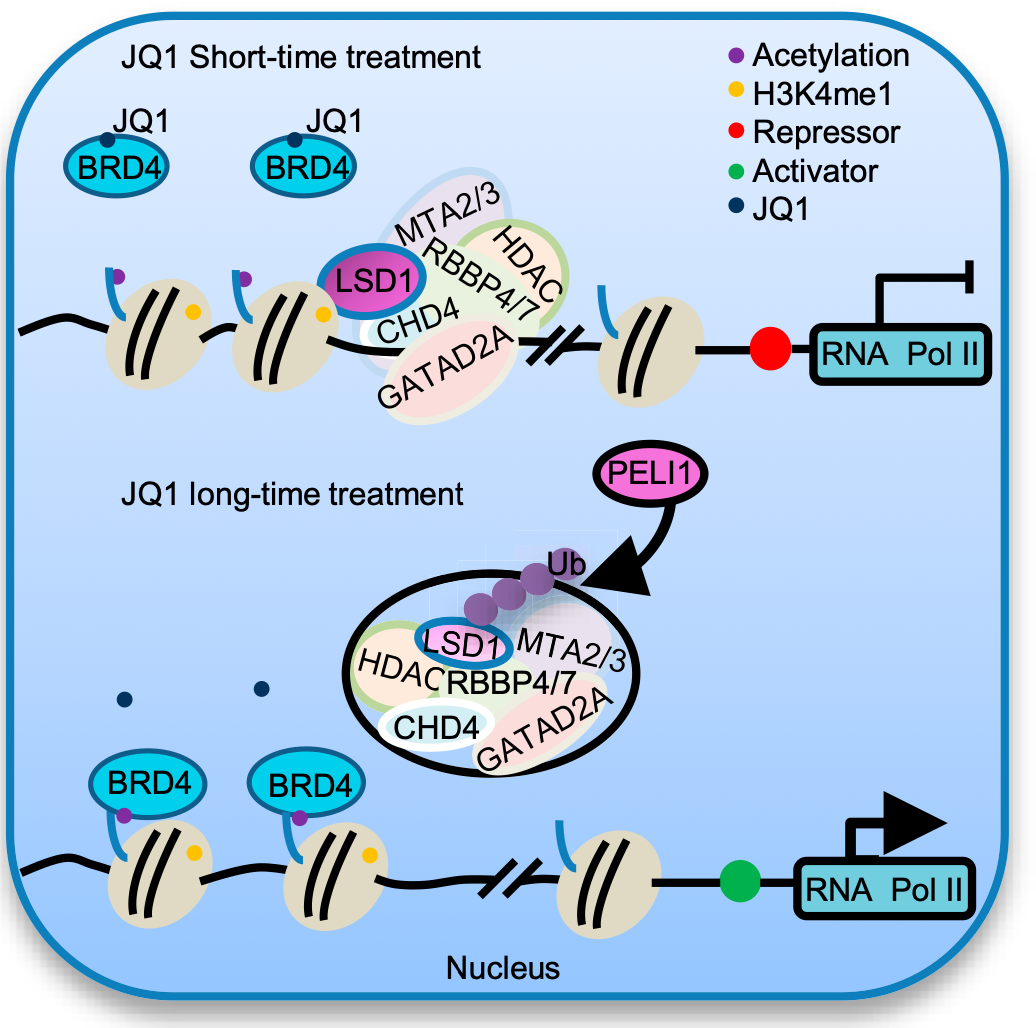
\includegraphics[width=0.3\textwidth]{../_resources/Screenshot_2022-10-28_at_11-55-04.png}
\caption{}
\end{figure}

Proposal: combined targeting of BRD4 and PELI1 as therapeutic for breast
cancer

\subsection{HSF2 cooperates with HSF1 to drive a transcriptional program critical for the malignant state}

Heat shock factor 1 (HSF1) is the master regulator of the heat shock response (HSR), a cytoprotective mechanism that induces expression of
molecular chaperones (HSPs), in response to multiple cues: environmental stresses, pathophysiological states, cell growth and development and
protein misfolding diseases.

In the context of cancer, HSF1 promotes gene expression of both canonical HSP target genes and of many non-canonical target genes with roles in diverse biological processes, beyond protein folding and stress responses, including include cell cycle and energy metabolism. In multiple types of cancer, HSF1 transcriptional program is associated with metastasis and a worst prognosis. HSF1 interacts with its paralog HSF2, physiologically involved in development, spermatogenesis and in the modulation of responses to select proteotoxic stresses, including proteasome inhibition, ethanol, and febrile-range thermal stress, rather than HSR. It is suggested that HSF2 can both promote and suppress cancer cell growth.

HSF2 strongly interacts with HSF1 in each of the four cell lines tested. \textbf{LUMIER assay} is a quantitative, high-throughput protein-protein assay able to capture transient interaction with high sensitivity in native conditions. LUMIER assay confirmed that HSF2 is the top HSF1-interacting transcription factor. Co-IP of endogenous HSF1 and immunoblot analysis of endogenous HSF2 were performed in a panel of cancer cell lines including breast, prostate, and lung cancer. Hence, \underline{HSF1 and HSF2 physically interact in cancer cells}. To explore the functional significance of this protein interaction in cancer cells, they performed an electrophoretic mobility shift assay (EMSA) to test whether HSF2 and HSF1 can each bind the canonical HSE in the promoter of HSPA8, bound by HSF1 with high affinity in cancer cells. HSF2 forms an active complex with HSF1, capable of binding DNA in proliferating cancer cells.

In addition, ChIP-seq analyses revealed that HSF2 shares chromatin occupancy sites with HSF1 in cancer cells, HSF2 is dispensable for HSF1 binding and HSF1 can promote HSF2 chromatin occupancy.

To investigate how HSF2 affects cancer cell gene expression and how this relates to HSF1 activity, they performed an RNA-seq on 11 aggressive
cell lines treated with siRNA for HSF1 or HSF2 or both. The analysis revealed five major clusters of differently expressed genes.

\begin{figure}
\centering
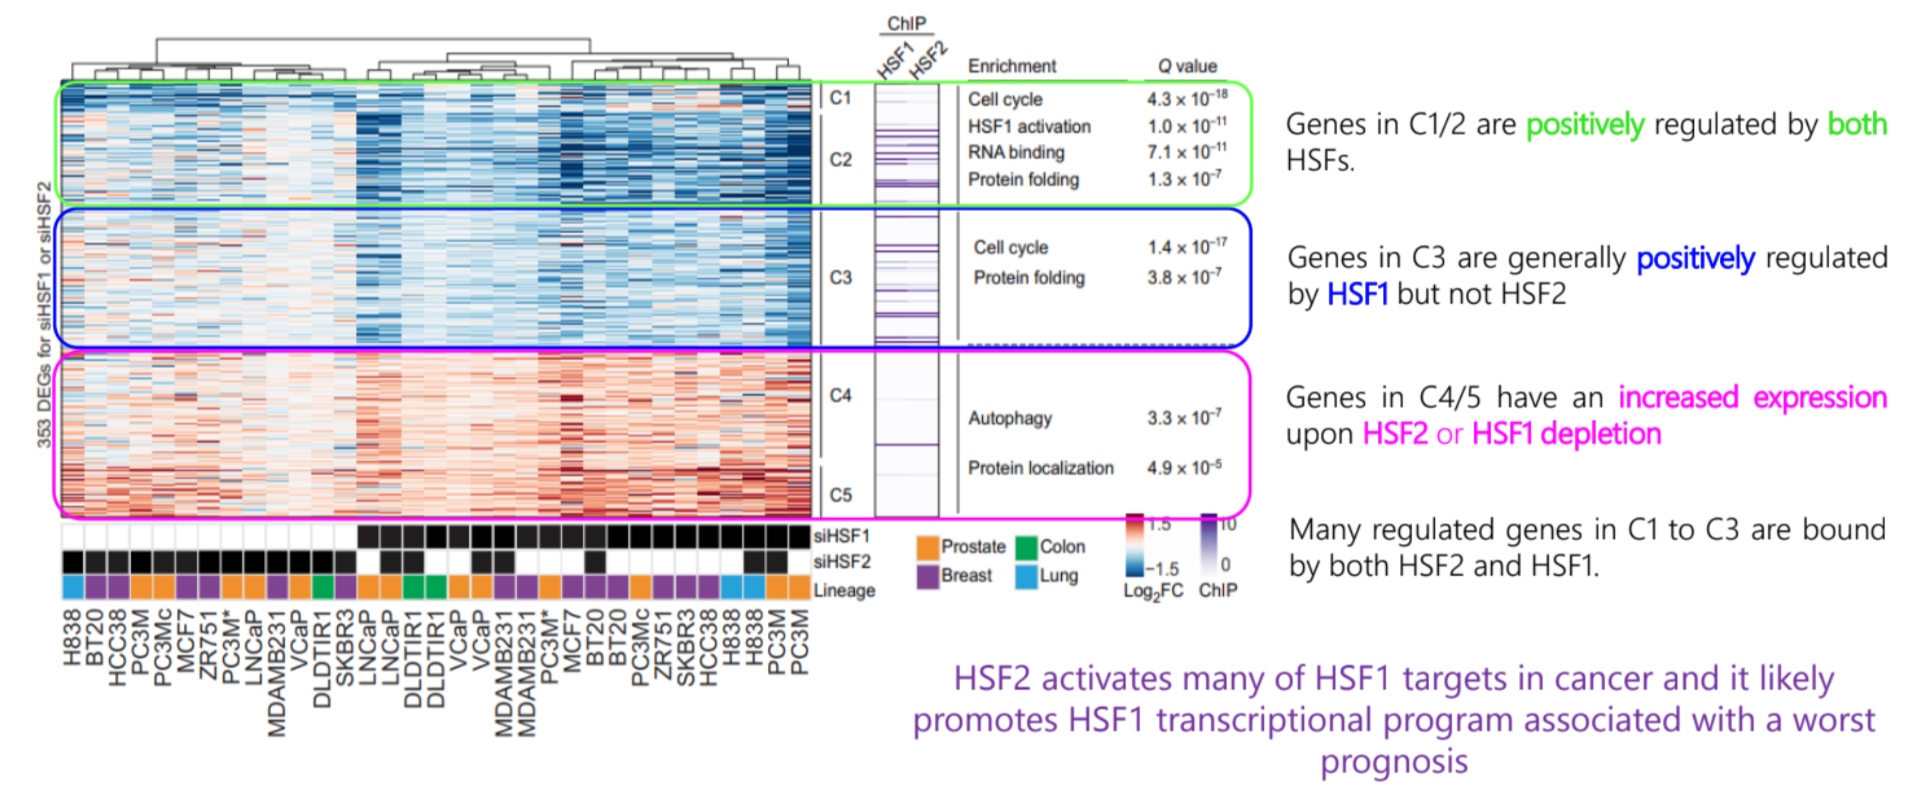
\includegraphics[width=0.8\textwidth]{../_resources/Screen_Shot_2022-12-20_at_11-45-23.png}
\caption{}
\end{figure}

While HSF2 and HSF1 drive expression of similar genes, the magnitude of changes on transcription with HSF2 depletion observed in cancer cells
was less than that of HSF1 depletion. HSF1 and HSF2 cooperate for maximal target gene expression. The formation of an HSF1-HSF2 complex drives concordant, direct regulation of many genes critical to the cancer gene expression programs.
The loss of either HSF provokes an adaptive change that is dependent on the cellular context. Loss of either HSF has durable consequences on gene expression with concordant decreases in the proteostasis gene expression programs. Since even in cancer cells with OE of HSF2, HSF2 loss didn’t alter the HSF1-dependent HSR, there must be a role for HSF2 that is other than the dispensable one in the HSR.
It is known that HSF1 plays a role in nutrient and oxygen and other stress responses, so it was tested if also HSF2 does MDA-MB-231 cells lacking HSF2, HSF1 or both were subjected to glycolytic stress (2-DG), serum starvation or the hypoxia mimetic CoCl2 (stabilizes HIF1-$\alpha$). The loss of either or both HSFs resulted in similar and broadly dysregulated transcriptional responses to these stresses.

\textbf{Conclusions:}
\begin{itemize}
\tightlist
\item HSF1 supports the malignant state by directing a transcriptional program of genes involved in many facets of tumorigenesis
\item HSF1 and HSF2 physically interact in cancer cells and HSF1 can promote HSF2 chromatin occupancy, abundance
and activity.
\item There is a strong pattern of chromatin co-occupancy, so phenotypes previously attributed solely to HSF1 may
reflect the effect of loss of both HSFs.
\item HSF1 loss reducing HSF2 expression and chromatin occupancy may contribute to the greater suppression of cell
cycle and proliferation-associated gene expression.
\item HSF2 loss alone could fall below a threshold of cytotoxicity that fails to result in severe growth arrest because of the
intact function of HSF1
\item HSF2 activates many of HSF1 targets in cancer to support the malignant state, associated with a worst prognosis, making HSF2, and HSF1-HSF2 complex, significant contributors in supporting cancer cell gene expression programs
\item The loss of either HSF provokes an adaptive change that is dependent on the cellular context, still, it was identified a core module of genes
with persistent reduced expression following HSF-KO across cell lines, comprising protein folding, DNA biosynthesis and stress response genes
\item The loss of either or both HSFs resulted in similar and broadly dysregulated transcriptional
responses to nutrient and oxygen stresses.
\item There is a critical role for HSF2 in directly regulating cancer response to metabolic stresses and tumor progression in cooperation with HSF1
\end{itemize}

This study has documented a significant role for HSF2 in supporting malignancy. Cancer-relevant stresses such as nutrient
deprivation or in vivo tumorigenesis invoke an HSF2-driven gene expression program, which parallels that driven by HSF1.
Thus, HSF2 is a critical HSF1 accomplice, promoting a gene expression program that supports the anabolic malignant state
and fuels cancer progression.

\subsection{Oncogenic lncRNAs alter epigenetic memory at a fragile chromosomal site in human cancer cells}
MANCA PRES SU DRIVE

Chromosome instability is a critical event in cancer progression. Histone H3 variant CENP-A plays a fundamental role in defining centromere identity, structure, and function but is innately overexpressed in several types of solid cancers. In the cancer background, excess CENP-A is deposited ectopically on chromosome arms, including 8q24/ cMYC locus, by invading transcription-coupled H3.3 chaperone pathways. Up-regulation of lncRNAs in many cancers correlates with poor prognosis and recurrence in patients. We report that transcription of 8q24-derived oncogenic lncRNAs plays an unanticipated role in altering the 8q24 chromatin landscape by H3.3 chaperone–mediated deposition of CENP-A–associated complexes. Furthermore, a transgene cassette carrying specific 8q24-derived lncRNA integrated into a naïve chromosome locus recruits CENP-A to the new location in a cis-acting manner. These data provide a plausible mechanistic link between locus-specific oncogenic lncRNAs, aberrant local chro- matin structure, and the generation of new epigenetic memory at a fragile site in human cancer cells.

\begin{figure}
\centering
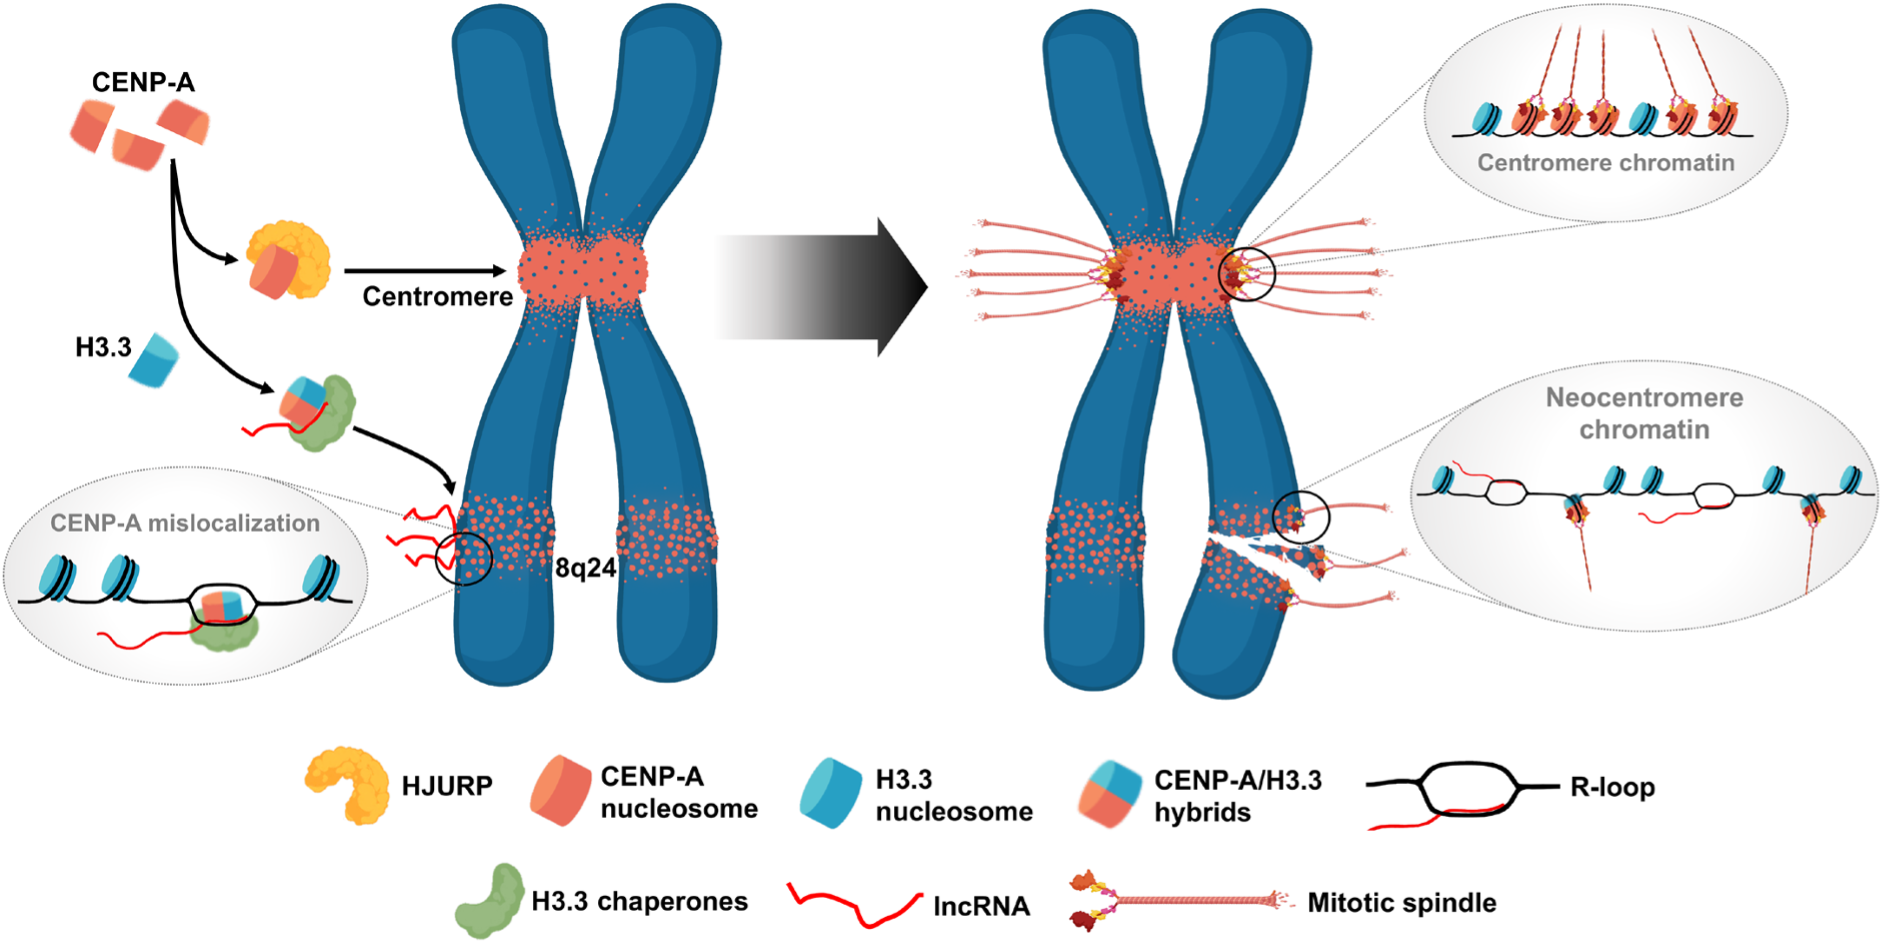
\includegraphics[width=0.7\textwidth]{../_resources/cenp.png}
\caption{Usually, CENP-A associates with its chaperone HJURP to deposit at centromeres. Overexpressed CENP-A in cancer cells possibly form hybrid nucleosomes with H3.3 and hijacks the H3.3 chaperone pathways to deposit ectopically, thus invading regions such as the 8q24 locus and altering the local chromatin landscape. The 8q24-derived oncogenic lncRNAs could serve as a recruitment signal for incorrect chaperone- histone variant complexes. The CENP-A at ectopic sites promotes active transcription of the local chromatin as a feedback mechanism, leading to a higher R-loop level. The R-loop tethered lncRNAs, in turn, could help CENP-A ectopic deposition. Further, the unresolved R-loop configuration with the ectopic CENP-A nucleosomes may impair DNA replication efficiency, resulting in an under-replicated DNA with stalled replication forks. When the cells enter mitosis amid chromosomes with decondensed chro- matin regions, with R-loops and ectopic CENP-A presence, these regions can build a weak ectopic kinetochore, resulting in chromosome breaks during segregation.}
\end{figure}

\section{Targeting transcription in cancer}
\subsection{Targeting histone acetylation dynamics and oncogenic transcription by catalytic p300/CBP inhibition}
P300/CBP are a transcriptional co-activators with lysine acetyltransferase. It localise to cis-regulatory elements in association with transcription factors. P300/CBP activity is linked to the physiological control of cell identity. Histone deacetylases have opposing enzymatic activity to P300/CBP, ensuring appropriate gene expression levels.
Some histone residue exhibit an acetylation-methylation equilibrium to fine-tune gene expression.
Unmodified H3K27  can be acetylated by P300/CBP or methylated by PCR2 repressor complex. The lysine is returned to its unmodified state by histone deacetylases or demethylases.

\textbf{Aim of the study:} use of catalytic inhibitors of P300/CBP to characterise the temporal epigenetic, transcriptional, and biological consequences of acute and sustained histone hypoacetylation.

P300/CBP inhibition showed rapid transcriptional modulation, with predominant downregulation of differentially expressed genes and significant preferential deacetylation of cis-regulatory enhancer elements. Chromatin accessibility remained unaffected following inhibition of P300/CBP using A-485 for 2 and 6h, despite transcriptional modulation and global histone hypoacetylation. 

Loss of H3K27ac and BRD4 binding at promoter regions predicted transcriptional sensitivity to P300/CBP inhibition and was associated with loss of RNA Pol II occupancy at gene promoters.

HDAC3-selective inhibitor RGFP966 mitigated histone hypoacetylation, but had limited effects on the acetylation of non-histone proteins.
Sustained H3K27 hypoacetylation is necessary to accumulate significant trimethylation levels. Acute and intermediate P300/CBP inhibition led to rapid reversion to an acetylated state. Histone methylation kinetics can augment p300/CBP.

\textbf{Conclusions:}
\begin{itemize}
\tightlist
\item Perturbation of the histone acetylation equilibrium resulted in transcriptional changes.
\item The reversibility of acute exposure to catalytic P300/CBP inhibition may increase the therapeutic index of non-covalent catalytic P300/CBP inhibitors in vivo
\item They demonstrated specificity of HDAC3 for the functional opposition of P300/CBP acetyltransferase activity.
\item Sustained histone hypoacetylation provides the nucleation point for the conversion to a stable trimethylated lysine.
\item KDM6A inhibition sensitise tumour cells to apoptosis mediated by P300/CBP inhibition.
\end{itemize}

\begin{figure}
\centering
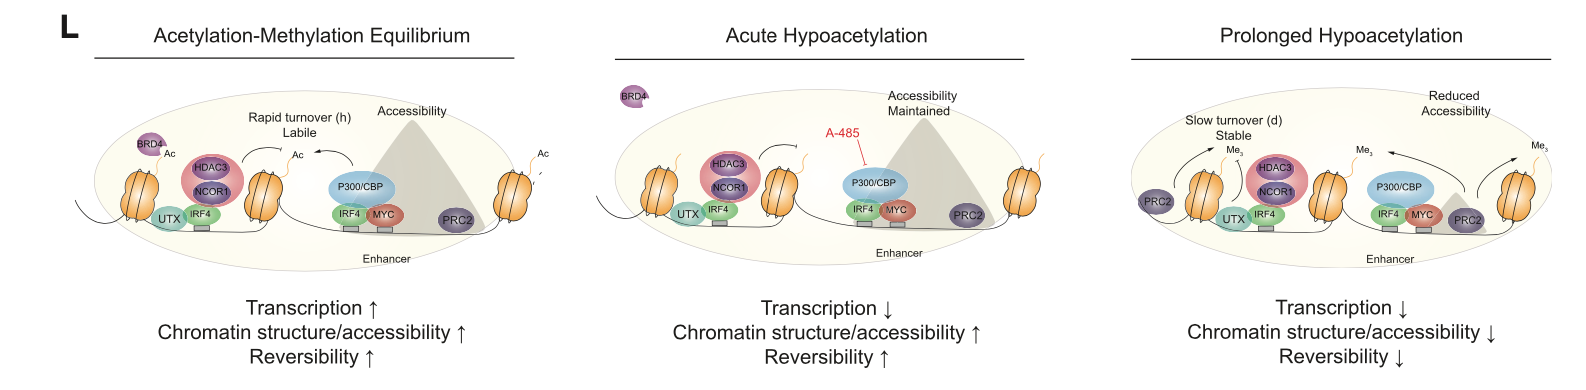
\includegraphics[width=\textwidth]{../_resources/Screen_Shot_2022-12-20_at_12-01-08.png}
\caption{Model for the temporal regulation of gene expression by the histone acetylation-methylation equilibrium and the consequences of KAT inhibition on cellular transcription independent of changes in 3D chromatin configuration.}
\end{figure}

\subsection{Super Elongation Complex as a Targetable Dependency in Diffuse Midline Glioma}
Soon after RNA Pol2 transcription starts it will recruit the
pausing factor DSIF and NELF, causing its pause.
The Super Elongation complex (SEC) or BRD4 complex acts as
a positive regulator of the release of RNA Pol2 from
promoter proximal pausing, allowing the productive
transcriptional elongation.

SEC complex is formed by:
\begin{itemize}
\tightlist
\item P-TEFb (CycT1-CDK9) → Catalytic subunit.
\item AFF4 → Scaffold Protein.
\item AF9/ENL → Interact with co-activators / co-
repressor.
\item ELL2 → Elongation Factor.
\end{itemize}

P-TEFb phosphorylates DSIF, NEL RNA Pol2 CTD at the Serine 2 causing its pause release.

\textbf{Diffuse Midliine Glioma} (DMG) arises in the glial cells of the brain’s midline
structures, especially the brainstem (midbrain,
pons, and medulla).  It is predominantly a pediatric disease, but it can
also occur in adults.
Curative surgery is not possible, radiation therapy
and chemotherapy provide only temporary relief.

It is defined by the presence of the H3K27M mutation.

\textbf{Aim of the study:} Identify specific epigenetic regulators that mediate the
altered developmental phenotype in DMG H3K27M+
transformed cell state.

Short hairpin RNA (shRNA) screen targeting 408 genes classified as epigenetic or chromatin-associated
protein revealred ssential genes for DMG cells, which were shRNA depleted.  DMG cells depend on the SEC component AFF4.

AFF4 and CDK9 knockdown led to a significant
decrease in proliferation across multiple patient-
derived H3K27M+ cell cultures.
Following depletion of AFF4, a decrease (-) in Myc and Myc dependent programs, increase (+) in neuroglia differentiation program
and diminished (-) capacity for self-renewal was observed. Hence, SEC play a role in maintaining a proliferative, stem-like state. CDK9i treatment effectively phenocopied the transcriptomic effects of AFF4 shRNA knockdown on differentiation programs.

H3K27M mutation perturbs the epigenetic regulation of AFF4 and may allow the aberrantly expressed SEC to contribute to DMG stem-like state maintenance.

Atuveciclib treatment on processive transcriptional
elongation induce targeting of pausing release
without targeting transcription initiation. ChiP-Seq of RNA pol2 upon atuveciclib treatment.
Clustering of genes by distribution of RNA pol2
occupancy:
\begin{itemize}
\tightlist
\item Absence of RNA pol2.
\item RNA po2 without downstream elongation.
\item Active RNA pol2 procession in the gene body
\end{itemize}
→ Genes involved in essential cellular
processes and neuroglia cell lineage.
In DMG, disordered SEC-mediated signaling may disrupt the context-dependent activation under which
pausing-regulated expression of neuroglial morphogenesis programs are regulated. This might be
reversed through CDK9i treatment.

Xenograft cohort receiving atuveciclib therapy
showed only modest survival benefit in
comparison to those receiving vehicle control.
Xenograft cohort treated with AZD4573
exhibited a more dramatic benefit to overall
survival and decreased tumor growth.
Anti-tumor activity demonstrated in orthotopic xenograft models of DMG using clinically relevant CDK9 inhibitors.

\textbf{Conclusions:}
RNAi screening approach to epigenetic regulation in
H3K27M mutant DMG to identify the SEC as a
targetable dependency.
SEC-mediated signaling appears to drive a
transcriptional program that contributes to DMG stem
cell maintenance and self-renewal.
Inhibition of this pro-oncogenic signaling via CDK9i
treatment restores promoter-proximal pausing of RNA
Pol2, promotes cellular differentiation programs and
prolongs survival in patient-derived xenograft models.

\begin{figure}
\centering
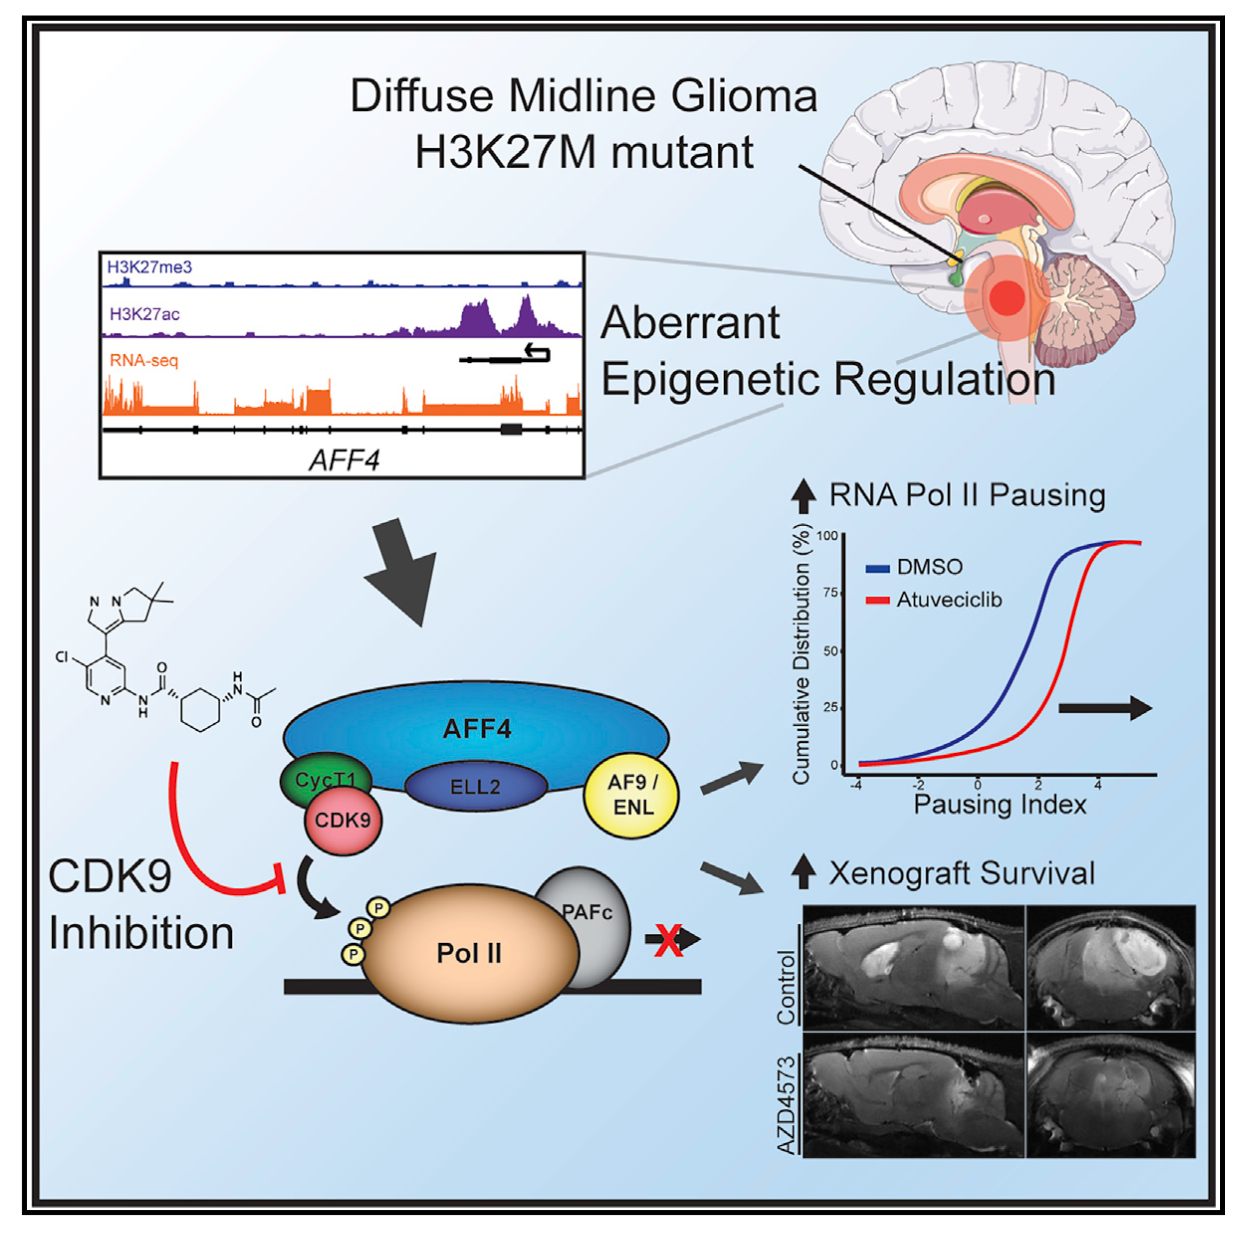
\includegraphics[width=0.4\textwidth]{../_resources/Screen_Shot_2022-12-20_at_12-43-26.png}
\caption{}
\end{figure}

\subsection{Transcription elongation factors represent in vivo cancer dependencies in glioblastoma}
Glioblastoma is the most common of all primary malignant central nervous system (CNS) tumors. Standard-of-care therapies consist of surgery, RT, and Temozolomide chemotherapy, but none of these are curative. It is thought to arise from neuroglial stem or progenitor cells and characterized by molecular heterogeneity. There are 3 main subgroups: proneural, mesenchymal and classic.

Pol II is initiated at the TSS and remains in the paused state until further stimulation ; p300/CBP is recruited and generates H3ac and/or H4ac. H3ac and/or H4ac recruits BRD4, which associates with 7SK snRNP/P-TEFb complex and JMJD6. \textbf{JMJD6} digests MePCE to disrupt the 7SK snRNP complex to release P-TEFb (CDK9). CDK9 phosphorylates Ser2 motifs on CTD of Pol II,  releasing it.

In vivo RNAi screening strategy was performed to enable the identification of chromatin regulators that are crucial for the survival of glioblastoma cells within a functional tumour microenvironment. Genes that caused cell depletion in both screens were restricted to the positive-control gene RPA3 and two genes essential for transcription and maintenance of DNA methylation, POLR2B and DNMT1. In vitro-specific hits were enriched for genes that promote cellular metabolism and macromolecule biogenesis, while in vivo-specific hits were enriched for genes controlling transcriptional elongation.

Gene expression profiles were markedly different when cells were grown in an intracranial xenograft model as compared to cell culture conditions. Cancer cells cultures were enriched for transcriptional programs of proliferation, whereas intracranial tumors were enriched for transcriptional programs of stress response, signalling response and other stimulus response pathways. Many upregulated genes in tumour cells grown intracranially were important transcription factors and signalling molecules regulated by polymerase II (Pol II) pausing. The upregulated genes were also highly expressed in tumours from patients with primary glioblastoma. The upregulated pause-controlled gene programs that occur in vivo may allow the tumour cells to interact with and adapt to their ­complex microenvironment, supporting their increased dependency on transcription pause–release and elongation factors for in vivo survival.

ChIP-Seq analysis of the enhancer mark H3K27ac revealed that the expression of the enhancers target genes corresponds to the condition-dependent changes in the enhancer signal, hence the microenvironment regulates the epigenome to transform the glioblastoma cell state by differentially activating enhancers and their target genes.

JMJD6 regulates many of the genes that are important for the survival of glioblastoma cells in vivo and may control transcriptional pause–release in primary glioblastoma tumours. Therefore, JMJD6 constitutes a strong lead target for further evaluation. JMJD6 may regulate the expression of genes targeted by JMJD6-bound enhancers through enhancer-mediated pause–release, both in the intracranial tumour environment as well as in patient tumours. JMJD6 binding is associated with increased enhancer activity and promotes pause–release in human glioblastoma cells within the tumour microenvironment.

Targeting of JMJD6 with an inducible shRNA distinct from the primary screen in vivo extended cell survival, so achieving sustained JMJD6 inhibition may provide a notable therapeutic benefit.

\textbf{Conclusions:}
\begin{itemize}
\tightlist
\item Developing and validation of a new in vivo functional screening strategy for glioblastoma that recapitulates most stressors and ­stimuli of the tumour microenvironment
\item Glioblastoma cells in vivo were dependent on Pol II pause–release and transcription elongation machinery for survival
\item Identification of several in vivo-specific biological targets for glioblastoma, including JMJD6
\item In the primary tumour, targeting the microenvironment-induced stress response mechanisms of the cancer cell may be a more effective therapeutic strategy than targeting cell growth
\end{itemize}

\begin{figure}
\centering
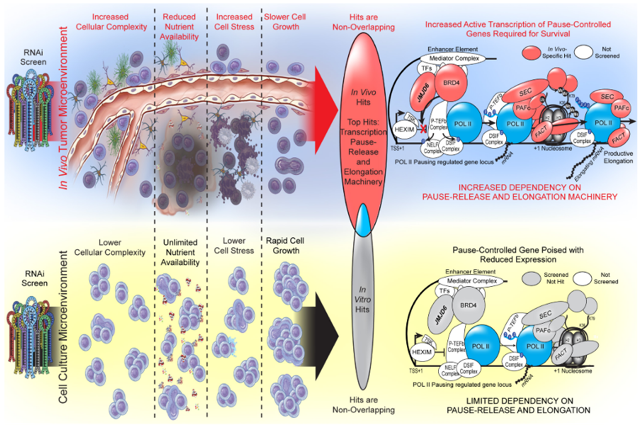
\includegraphics[width=0.6\textwidth]{../_resources/RNAi.png}
\caption{}
\end{figure}

\section{Nuclear receptors in cancer}
\subsection{ER$\alpha$ is an RNA-binding protein sustaining tumor cell survival and drug resistance}
Nuclear receptors are a family of 48 TFs expressed along the body. Most of them bind lipophilic ligands.
Structural changes enable their transcriptional activity, allowing a rapid respond to environmental stimuli.
The estrogen receptor is codified by ESR1 gene. 15-20\% of breast tissue cells are ER+ and  ~75\% of breast cancer are ER+ 

ER$\alpha$ protein interactome was analysed through IP followed by MS; RNA binding proteins was the most enriched category. By performing CLIP (Cross-linking and IP) method, ER$\alpha$ was found to be RBP associated with multiple oncogenic mRNAs.  ER$\alpha$ directly binds RNA
Binding occurs preferentially at 3’UTR region for genes involved in cancer progression events, apoptosis, cell growth and motility.

RNABindRPlus tool was used to predict RBD binding sequence, which was identified between 255-272aa within the \emph{hinge domain}. RNA-binding domain mutation impairs ER$\alpha$-mRNAs association and RBDmut ER$\alpha$ can localize to the nucleus, without affecting DNA-binding ability. It was seen that ER$\alpha$ is essential for cancer cell growth.

CRISPRi screening allowed the identification of transcripts whose silencing impairs cell growth. Gene Ontology Analysis to classify these genes  adaptive response to stress. 
mRNAs bound by  ER$\alpha$ are essential for breast cancer fitness:
\begin{itemize}
\tightlist
\item MCL1: anti-apoptotic protein myeloid cell leukemia 1
\item elF4G2: eukaryotic translation initiation factor 4 gamma 2
\item XBP1: Transcription factor X-box binding protein
\end{itemize}
ER$\alpha$ RNA-binding facilitates XBP1 splicing upon stress and ER$\alpha$  modulates the translation of eIF4G2 and MCL1 mRNAs

ER$\alpha$-regulated genes are overexpressed in tumor samples with respect to adjacent tissue.
Targeting ER$\alpha$ post-transcriptional signaling abrogates cell survival and reverses tamoxifen resistance.

\textbf{Conclusions:}
\begin{itemize}
\tightlist
\item ER$\alpha$ is a master transcription factor controlling breast cancer progression
\item ER$\alpha$ role as RBP in adaptive response to stress against endocrine therapies 
\item Translational control on MCL1 and eIF4G2
\item Alternative splicing of XBP1
\item New therapeutic window for treating breast cancers, intervening on post-transcriptional regulation
\item ER$\alpha$+ breast cancers may be sensitive to therapies against stress response 
\end{itemize}

\begin{figure}
\centering
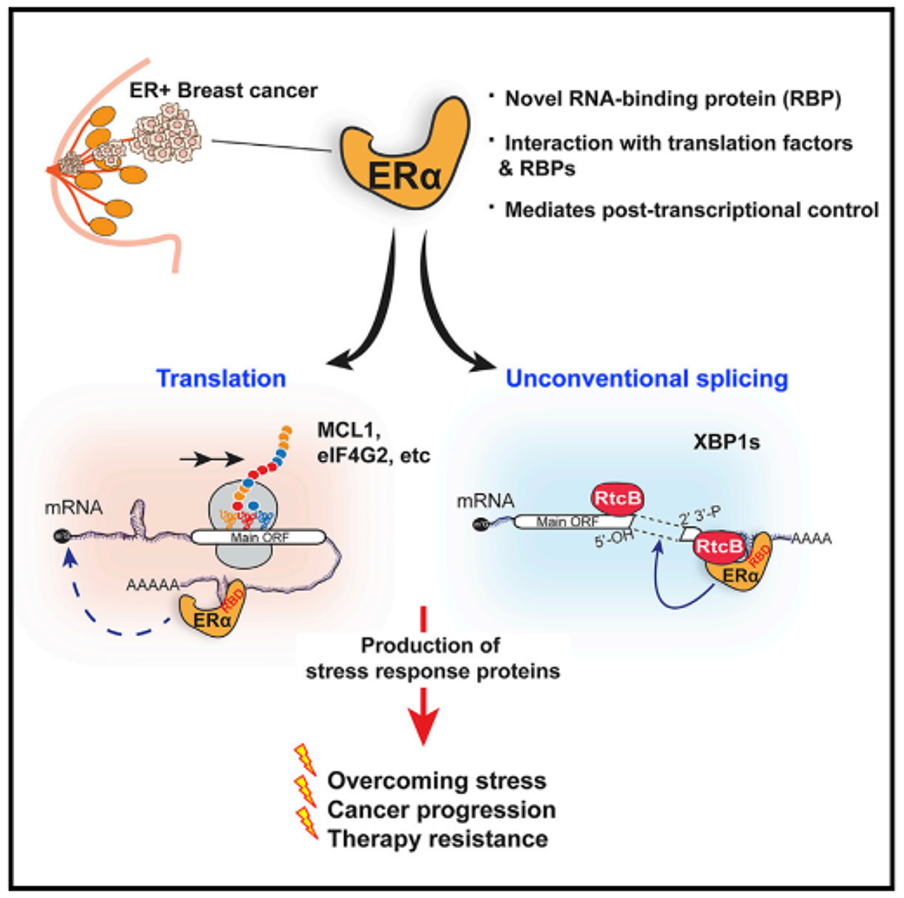
\includegraphics[width=0.3\textwidth]{../_resources/era.png}
\caption{}
\end{figure}

\subsection{Analysis of estrogen-regulated enhancer RNAs identified a functional motif required for enhancer assembly and gene expression}
Enhancers are characterized by common molecular features, such as: 
\begin{itemize}
\tightlist
\item Open or accessible chromatin environment 
\item Enrichment of a common set of histone modifications, like H3K4me and H3K27ac 
\item Binding of transcription factors, coregulators and chromatin remodelling enzymes 
\item Looping to target gene promoters  
\item Production of enhancer RNAs (eRNAs)
\end{itemize}

eRNAs are often non-polyadenylated and are sometimes capped.  They are difficult to study due to their short half-life. 
How to study eRNAs? 
\begin{itemize}
\tightlist
\item Loss of function approaches $\rightarrow$ siRNAs 
\item Gain of function approaches  $\rightarrow$  eRNA plasmid mediated over-expression
\end{itemize}

After the creation of a RNA sequencing library using polyA depleted and polyA enriched fractions
isolated from ER+ MCF7 cells, two different approaches were exploited for eRNA annotation: StringTie followed by filtering based on the overlap of transcripts with intergenic ER$\alpha$ binding sites and PROcap approach to identify the transcription starting site of eRNAs.
1023 E2-regulated eRNAs in the polyA-depleted fraction and 213 E2-regulated
eRNAs in the polyA-enriched fraction were identified.
These eRNAs tend to be short (449nt on average) and their TSS present an enrichment for the Initiator element.

They classified ER$\alpha$ enhancers into three groups:
\begin{enumerate}
\tightlist
\item ER$\alpha$ binding without enhancer transcription
\item ER$\alpha$ binding with enhancer transcription but
no detectable eRNAs
\item ER$\alpha$ binding with both enhancer transcription
and eRNAs
\end{enumerate}

Upon targeting eRNAs to their cognate
enhancers, it is possible to observe a
shortened expression timescale and an
augmented expression of target genes in
response to E2 treatment.
This suggests a functional role for eRNAs in the context of E2 treatment.
By targeting eRNAs to non-cognate enhancers, no
increase in target gene expression is visible.
This suggests that eRNA tested are not
interchangeable and may rely on locus-specific features for their activity.

eRNAs did not exert their activating effects at enhancers in absence of E2 treatment and eRNA alone construct was insufficient to enhance target gene expression, suggesting that these.
eRNAs are unable to function outside their native genomic context and not every eRNA tested affected target gene expression.
Not all the genes sharing a TAD with the enhancer showed enhanced expression upon eRNA
targeting.

Collectively, these results demonstrate that some of the eRNAs tested act in cis at their enhancers of origin and
modulate functional outcomes, such as shortening the timescale
and increasing the magnitude of target gene expression upon E2
treatment and the eRNAs tested are not interchangeable and may rely on locus-
specific features for their activity.

ChIP qPCR revealed that kinetics of enhancer
activation vary from enhancer to
enhancer. Thus, different enhancers
behave differently. Upon p300 inhibition there is an inhibition of the eRNA mediated H3K27ac.
Together, these results demonstrate that selected eRNAs, when
recruited to their enhancer of origin, can increase the recruitment of
ER$\alpha$ in response to E2 treatment and stimulate H3K27 acetylation in
cells. These effects, however, occur in a locus-specific manner,
suggesting additional locus specific features for their activity.

MEME+FIMO  $\rightarrow$  \textbf{FERM} element, forming a hairpin structure in both PRRX2 and UBE2E. Introduction of two FERM elements on
sgRNAs of the two sistems showed enhanced target gene transcription as well as enrichemnt in ER$\alpha$ binding and H3K27ac.
FERM element is capable of stimulating target gene expression by
modulating the recruitment of ER$\alpha$ to its enhancer and stimulating
p300- catalyzed H3K27 acetylation in locus-specific assays.
While the FERM elements in tethered eRNAs may act to enhance
enhancer activity, they do not contribute the enhancer specificity of
eRNAs that we observed.

RNA-protein pulldown analysis coupled with mass spectrometry revealed 88 proteins enriched in
FERM element. Among tese proteins there is BCAS2, an RNA-binding component of the spliceosome, that
intercats with ER$\alpha$ and functions as a coregulator. \textbf{BCAS2} is an eRNA- and FERM-binding protein that plays a role in the eRNA- and
E2-mediated stimulation of target gene expression, ER$\alpha$ binding at the
enhancer, and eRNA- and FERM-mediated H3K27 acetylation.  Results suggest a role for BCAS2 in regulating ERa enhancer formation and subsequent gene expression, as well as a role for eRNAs in driving biological responses, including gene expression and
cell proliferation in breast cancer.

\textbf{Conclusions:}
\begin{itemize}
\tightlist
\item Results demonstrate that eRNAs targeted to their enhancer of origin require E2 function. This can be
explained by the fact that E2 stimulates ER$\alpha$ binding to chromatin, and liganded DNA-bound ER$\alpha$
recruits coregulators and RNA pol II to initiate eRNA production. Thus, eRNAs do not function on an
empty enhancer but on liganded ER$\alpha$ –bound enhancer reinforcing ER$\alpha$ binding and coregulator
recruitment in a virtuous cycle.
\item Some of the tested eRNAs promote the recruitment of ER$\alpha$ to enhancers and stimulate p300 activity
to increase HK27ac. It has been recently demonstrated that p300 is able to bind eRNAs through its
histone acetyltransferase domain and this stimulates its catalytic activity.
\item The presence of an eRNA at the enhancer in absence of E2 is sufficient to stimulate the activity of
pre-bound p300, but it is insufficient to drive the binding of ER$\alpha$ and subsequent recruitment of
cofactors. Indeed, treatment with p300 inhibitor decreased H3K27 ac levels even without E2
stimulation, indicating that there is a basal p300 catalytic activity.
\item They discovered the presence of FERM element in the tested eRNAs, which is sufficient to drive
E2-regulated target gene expression.
\item FERM element stimulates p300 catalytic activity and mediates interactions with BCAS2. These
functions could be regulated at many enhnacers across the genome, but the specificity of eRNAs
for their cognate enhnacer suggests that the non-FERM portions of the eRNA act to direct FERM
element to specific enhnacers.
\item Data demonstrates that an eRNA can act at an oncogenic enhancer to enhance oncogene
expression in breast cancer cells to increase cell proliferation. Further studies are needed to
better characterize how eRNAs modulate target gene expression and regulate enhnacer
formation and to elucidate the tehrapeutic potential of targeting eRNAs in breast cancer.
\end{itemize}

\begin{figure}
\centering
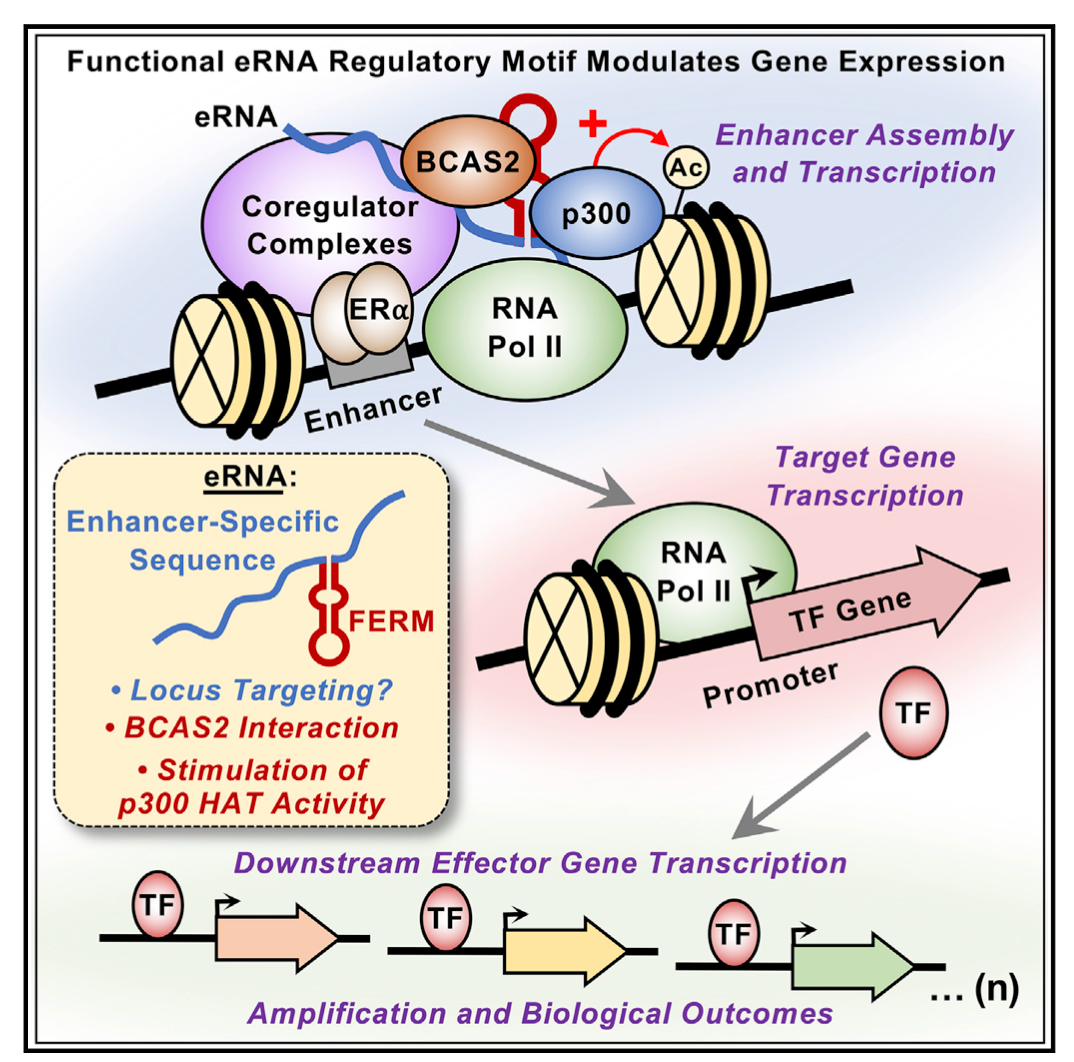
\includegraphics[width=0.3\textwidth]{../_resources/Screen_Shot_2022-12-20_at_14-17-02.png}
\caption{}
\end{figure}






 


